%!TEX root = paper.tex
%%%%%%%%%%%%%%%%%%%%%%%%%%%%%%%%%%%%%%%%%%%%%%%%%%%%%%%%%%%%%%%%%%%%%%%%%%%%%%%%
\section{Background}
\label{sec:background}

Some fundamental gaming terms and concepts need to be introduced first.


%%%%%%%%%%%%%%%%%%%%%%%%%%%%%%%%%%%%%%%%%%%%%%%%%%%%%%%%%%%%%%%%%%%%%%%%%%%%%%%%
\subsection{Basic Game Model}
\label{subsec:game-model}

At their core video games are essentially feedback-directed real-time simulators. Figure~\ref{fig:gameloop1} overviews a simplified simulation loop consisting of three parts. The game reads player input, updates the game state, and renders new screen contents. This loop repeats as long as the game is running. While the three parts are interrelated, and every component provides some form of input to the next, they may still proceed at their own intrinsic paces.


\begin{figure}[!t]
	\centering
	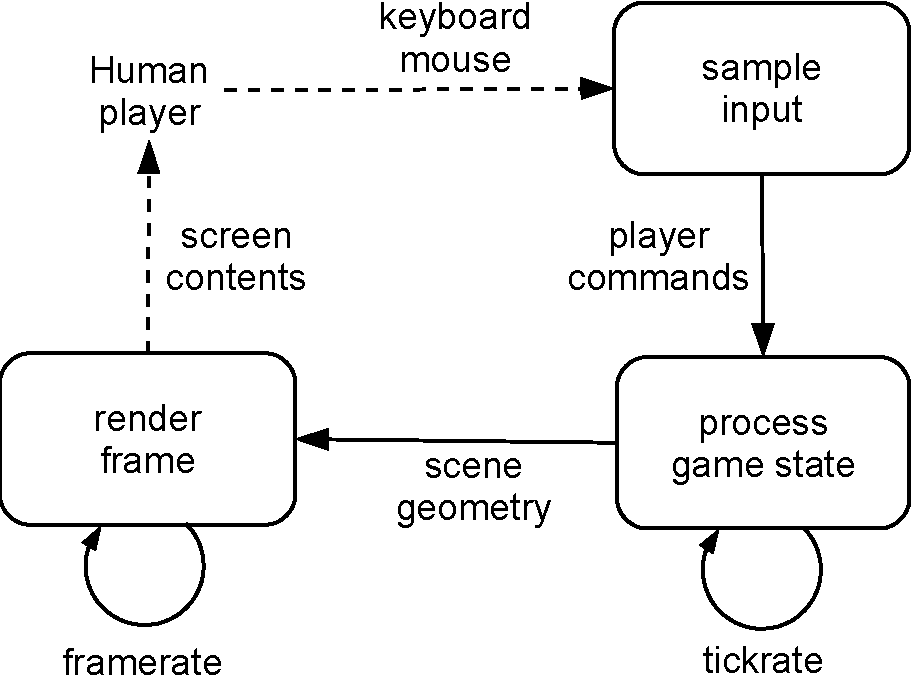
\includegraphics[width=0.8\columnwidth]{../../../models/game_loop.pdf}
	\caption{Basic model of a continuous main video game loop.}
	\label{fig:gameloop1}
\end{figure}

For example, the state of the game world is updated even if the player character does not move. In this simplified model, we distinguish a generic process for player input, a \textit{tickrate} that governs the frequency of game state updates, and a \textit{framerate} determining how often the screen is updated every second. The \textit{tickrate} governs the frequency of game state updates, and the \textit{framerate} determines the update rate of the output image. This basic makeup can be found in almost any kind of game architecture.
%of which three are depicted in Fig.~\ref{fig:component-models}.
The game server in client/-server games is the single authoritative point of state synchronization for other connected clients. Peer-to-peer architectures are not investigated here. Player input events are usually also only sent to the server according to a specific clocked \textit{command message rate}.

% \begin{figure}[!t]
%   \centering
%   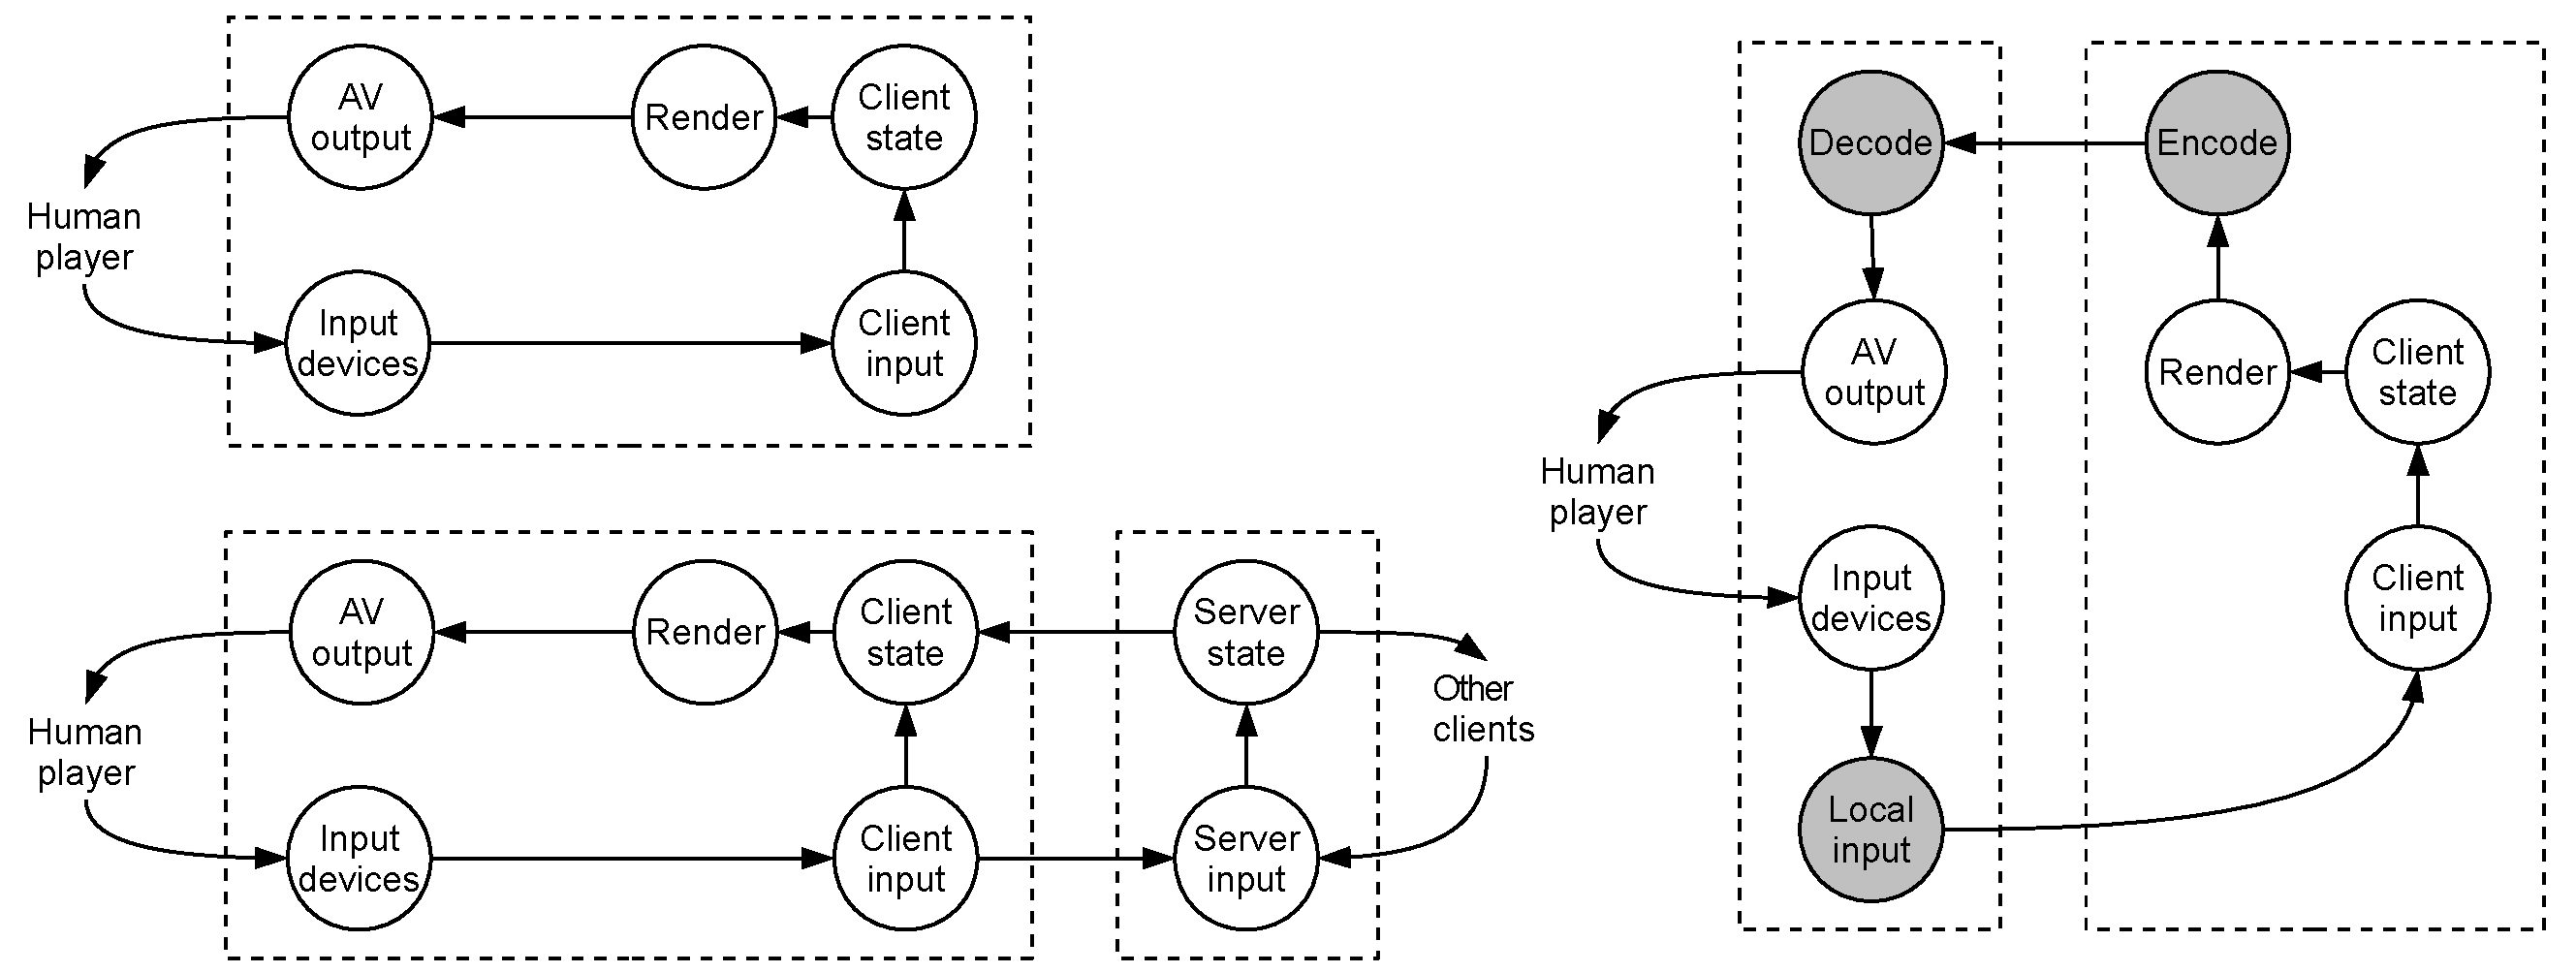
\includegraphics[width=0.9\columnwidth]{../../../models/component_interaction_full.pdf}
%   \caption{Interactions between components in different video game models. \textit{(a)} Single-player, \textit{(b)} online, \textit{(c)} cloud game.}
%   \label{fig:component-models}
% \end{figure}

Note that actual game implementations sometimes choose to update parts of the game state on different fixed frequencies. For example, a physics effect that does not influence gameplay directly could be updated at only half the tickrate. Also, the parameters of the player input process depend on the game genre and on the player action currently performed. Examples for the tickrates of popular networked games and their servers include \SI{64}{\hertz} or \SI{128}{\hertz} for \textsc{CS:GO}, \SI{20}{\hertz} for \textsc{Minecraft}, or \SI{30}{\hertz} for \textsc{Dota 2}.


%%%%%%%%%%%%%%%%%%%%%%%%%%%%%%%%%%%%%%%%%%%%%%%%%%%%%%%%%%%%%%%%%%%%%%%%%%%%%%%%
\subsection{Framerate}
\label{sec:framerate}


Below the threshold of \textit{apparent motion} (about $16.67$ frames per per second) objects will appear as two distinct objects between two consecutive still images. Video games are more flexible but also much more demanding on the framerate than traditional media, whose framerates hover at the lower end of motion perception. Video games have to target higher framerates, e.g., \SI{30}{\hertz}, \SI{60}{\hertz}, or even \SI{120}{\hertz}. This enables smoother camera and object movement and help increase the interactivity and reactivity as video games constantly require input on short time scales to which the game reacts and displays the feedback.


In contrast to traditional video media that play back at fixed framerates, e.g., \SI{24}{\hertz}, video games are more flexible but also much more demanding on the framerate. First, the framerate in a game may fluctuate as the processing time of the render process depends on the scene complexity. Then, video games usually target higher framerates than other media do: \SI{30}{\hertz}, \SI{60}{\hertz}, or even \SI{120}{\hertz}, depending on the type of game. Higher framerates enable smoother camera movement and scene transitions, as games often present faster scenes when compared to videos; they also help in increasing the interactivity as video games constantly require input on short time scales to which the game reacts and displays the feedback. Therefore, the framerate influences the reactivity of a game, but can also be a source of latency itself.

%%%%

%%%%%%%%%%%%%%%%%%%%%%%%%%%%%%%%%%%%%%%%%%%%%%%%%%%%%%%%%%%%%%%%%%%%%%%%%%%%%%%%
\subsection{End-to-End Lag}
\label{sec:e2e-lag}

Lag in video gaming is often described solely on the basis of the network delay in an online game. It should be evident that the lag is a critically important factor for almost all games, as it governs the reaction time to in-game events.

However, focussing solely on network delay neglects other components that contribute to the lag, including the input device, the time to sample and process the input, the game engine and server and their tickrates, frame rendering time, and ultimately the time to display the frame on the monitor. Only if all sources are factored in the complete \textit{\gls{E2E} lag} is captured. Notably, this lag is usually not constant but can vary depending on the type of action triggered by the input. While some simple actions, say opening the menu, may have a very short lag, more complex interactions, e.g., issuing command that moves the player character in the game world, may take considerable longer to complete. %, partly due to the actions taking more than one game tick to complete.
Therefore, each video game will have a distinct ``lag profile''.

% Fig.~\ref{fig:measurement-methods} depicts three distinct vantage points to measure portions of \gls{E2E} lag. Only external methods can capture the complete lag.

% \begin{figure}[!t]
%     \centering
%     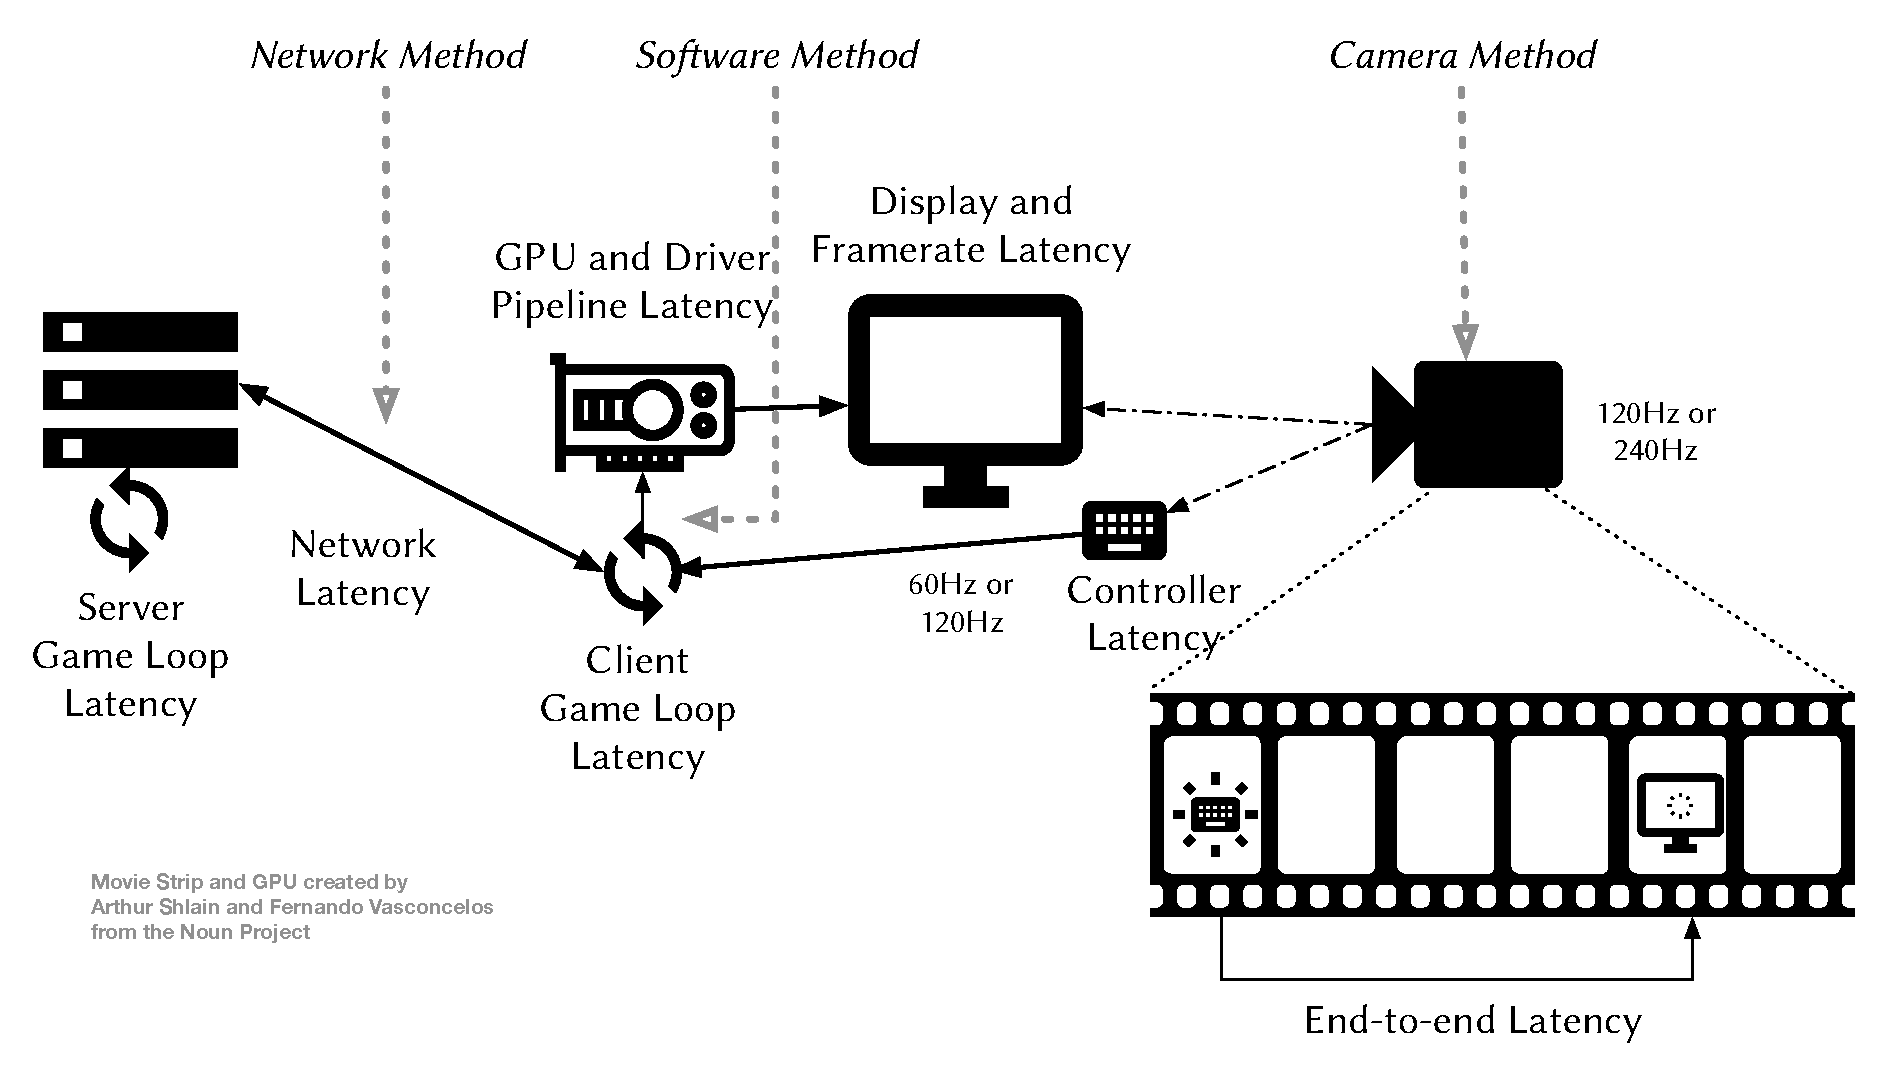
\includegraphics[width=1.0\columnwidth]{../../../models/e2e-lag.pdf}
%     \caption{Location of three measurement approaches to capture end-to-end lag in an online video game.}
% \label{fig:measurement-methods}
% \end{figure}



%%%%%%%%%%%%%%%%%%%%%%%%%%%%%%%%%%%%%%%%%%%%%%%%%%%%%%%%%%%%%%%%%%%%%%%%%%%%%%%%
\subsection{Related Work}
\label{sec:relatedwork}

The outcome of user studies in gaming depends on a wide selection of factors, e.g., on the precise setup, the game, and the choice of players. This makes comparing their results quite difficult.

In \cite{5976180} Jarschel et al. identify some influence factors on the subjective quality of cloud gaming through a user survey for certain games and three different game categories (slow, medium, fast games) that have been subjected to worsening \gls{QoS} parameters. Downstream packet loss and delay was noted be be especially problematic for achieving a good quality. Similarly, the authors of \cite{4591393} observed the relationship of players quitting a \gls{MMO} game with deteriorating \gls{QoS}. Additionally, a user study in \cite{4604397} also showed a correlation of the \gls{QoE} to the delay as well as the jitter for another \gls{MMO}, in this case the total delay had more impact than the delay variation. Regarding the subjective quality in first person shooters, the authors of \cite{6614351} find a strong impact of the delay and packet loss on the experienced quality. An ITU-T Recommendation \cite{mollertowards} concerning subjectively measuring video game \gls{QoE} is also in preparation, which discusses game-relevant \gls{QoS}-metrics as well as the selection of players and games.

Other approaches examine the player objective performance through in-game metrics such as the game's highscore or the duration to achieve a certain task. A 2006 paper \cite{Claypool:2006:LPA:1167838.1167860} categorizes player actions and their relationship to latency, with special regards for the precision and deadlines of actions. The ``kills per minute'' of players in the \gls{FPS} \textsc{Quake 3} are, for example, investigated by \cite{1266180}, which sees a steady decline of this subjective performance metric when increasing the network delay. A further paper \cite{claypool2007} notes the influence of network \gls{QoS} on in-game actions and specifically looks at player performance in first person games, with the performance being worse in a degraded network. Finally, the authors of \cite{Bredel:2010:MSR:1944796.1944797} also find a strong and negative influence of high delay on the player's performance, in this case again in \textsc{Quake 3}. 

On a more fundamental level, Ivkovic et al. \cite{Ivkovic:2015:QMN:2702123.2702432} quantify the effect of local latency, including input, rendering, and output devices. They find that as the latency is increased from 11 to 164 ms, the time-to-completion for 3D targeting tasks increases by around 50\% from 0.4 and 0.8 seconds for ``easy'', i.e. larger, and ``difficult'' targets respectively. The time the test subjects succeeded tracking a moving target reduces by 30\% as the latency is increased. These results are qualitatively similar to a much earlier study \cite{Ware:1994:ROV:198425.198426} on the difficulty of reaching for static objects in Virtual Reality displays, conditioned on the virtual object's size and the motion-to-display lag.


% \begin{table}[!t]
% \caption{Tickrates in competitive and popular video games that are either known, speculated upon, or derived by counting update and command messages. Data was collected from various sources and should be taken as-is.}
% % \hoss{Welche rel. bzw. unreliable sources? Gibt es auch typische framerates dazu?}
% % fm: inoffizielle, nicht-wissenschaftliche quellen, da diese werte normalerweise nicht durch den entwickler veröffentlicht werden; für framerates gibt es keine werte, da diese normalerweise unlocked laufen (zumindest für pc, bei konsolen für alle entweder 30 oder 60), ist eigentlich zu komplex um an der stelle darauf einzugehen
% \label{tbl:tickrates}
% 	\centering
% 	\begin{tabu}{X[0.45]X}
% 		\toprule
% 		\textbf{Video Game} & \textbf{Tickrate} \\
% 		\midrule
% 		CS: GO & Configurable \SI{64}{\hertz}/\SI{128}{\hertz} \\
% 		Battlefield 4 & \SI{30}{\hertz}; \SI{10}{\hertz} for state outside of close proximity to player; \SI{60}{\hertz}/\SI{120}{\hertz} on test servers. \\
% 		Minecraft & max. \SI{20}{\hertz} \\
% 		League of Legends & \SI{30}{\hertz} (estimated) \\
% 		Dota 2 & \SI{30}{\hertz} \\
% 		StarCraft II & supposedly either \SI{16}{\hertz} or \SI{32}{\hertz} \\
% 		Eve Online & \SI{1}{\hertz} \\
% %		Sports Game 1 & \\ \midrule
% 		Project Cars & \SI{600}{\hertz} (Physics), \SI{250}{\hertz} (Input) \\ %https://twitter.com/projectcarsgame/status/551340759858040833
% 		\bottomrule
% 	\end{tabu}
% \end{table}
